\chapter{User Interface Design}
\section{Overview and Introduction Screens}
When I started designing the user interface, I had set myself the goal of making the use of the app as intuitive as possible, so that it would take as less effort as possible from the user to get to learn the interface and how to use the application.

I also started thinking about how I was going to tackle the implementation of the data in the system and how to make the application do all the things that I had planned for it to do.

When I was planning the application and the features that it would have, I was planning with the vision of it being used by a single person for personal use and since the application didn't hold any information that would be valuable to steal, such as credit card numbers or bank account numbers, that it wasn't necessary to implement any supplementary security measures other than the ones that users implement in Android itself (such as screen lock) or to create any accounts to access the application.

However, I knew that I wanted the application to ask the user for certain data when lauching the application for the first time in order to get a base for the rest of the functionality. I planned then for the application to have three introductory screens:

\begin{itemize}
  \item An introduction saying the information that would be required from the user in order to get the application running
  \item A screen to enter the initial budget seperated by categories
  \item A screen to enter the monthly income of the user
\end{itemize}

\section{Home Screen and Expenses-related screens}
After deciding on what the introduction screens would contain, I started thinking about what the user would want to see when they would enter the application every single time in the form of a home screen. Since the goal of the application was to encourage the user to enter their expenses on a daily basis, I decided on making the home screen display the expenses that the user has made on the current day, as well as the money that the user has left until the next pay check and for the day and to let the user add expenses to the system with the help of a button clearly displayed on top of the list of expenses for the day.

When I was thinking of a way to list the expenses, I had to make a decision on what kind of information I wanted the expenses to contain. I came to the conclusion that since the expenses would be entered by the user into the system, that they would want to give them a name, as well as a description in case the expense contains many things (for example, when doing the shopping for the week), but also that some more basic information should be associated with them, such as the store or place where the expense was made, to which category it belonged and how much it was. That was quite a lot of information to be contained inside a home screen. In order to unclutter the home screen and make the information as accessible as possible to the user but still allow them to see the most important information, I planned on making the elements in the list of expenses clickable, and, when clicked, lead the user to another screen that would then display all the information of the expense to the user in a clear and concised way.

After making that decision, I had then to decide which data to present to the user in the expenses list. When designing the sketches and wireframes, I had in mind to present the name of the expense, the place where it was made and the amount of money,but, due to constraints inside App Inventor, what I ended up implementing was only the name and amount of the expense.

After deciding what the home screen would contain, I was left with the dilema of how to manage navigation inside the application. For that purpose, I had different options, such as a collapsible menu or a navigation bar. I decided to implement a navigation bar that would lead the user to the main functions of the application, and then inside the main pages, if necessary, lead the user to additional screens through buttons or list elements, just like for the expenses list on the main page or the button to add expenses.

After designing the home screen, I started designing the view that would display the information for an expense. My goal for that view was to give as much space for the display of information as possible and to present it clearly and properly separated so that the user could grasp it easily. When designing it, I made sure that the user also knew what was the information that was presented to them by the means of labels explaining what the following information was. I also wanted the user to be able to do something with that page other than consult the information related to that expense, so I planned on adding two buttons at the button of the screen, one that would allow the user to modify the information of that expense and another to delete the expense from the system. In the final product, however, considering that the user can add an expense to any date they wish, I decided to remove the modify button from that screen and only leave the delete button.

The next screen that I designed was the screen to add expenses. My intent with that screen was to make it in the shape of a form. An horizontal space would be reserved for each of the information required from the user for the expense, allowing the screen to not be overflowed with elements, and at the right bottom of the screen would be a button for the user to save the information in the system.

\section{Button placement}
Since I just evoked buttons and their placement, I have placed most of the buttons in the application on the firstly on the bottom of the screen but then also to the right of the screen since most people are right-handed and tend to hold their phone only with their right hand and use their thumb to interact with the screen.

\section{Category-related screens}
For the categories views, I decided to use a similar approach to the one for the expenses views. The user would be able to see a list of the categories and the amount of money that has been allocated to each of them thorugh a list on a categories main page that would be accessible though the navigation bar. Clicking on any of the items of the list would then lead to a page with the details of the category and a button that would lead the user to a page displaying all the expenses that were assigned to that category in a list, just like the one from the home screen.

The view presenting the user with the details for the category would be very similar to the one displaying the details for an expense, and would also allow the user to change the amount of money allocated to that expense. Some of the information displayed for that category would also be what should be associated type of expenses should be associated with that category and an estimate of how much of the income should be allocated to said category, according to \emph{enter reference here}.


\section{Budget, Income and Settings views}
The last views that I designed were the views for the budget, the income and the settings.

The budget view allows the user to both check and change the amount of money that is set to be spent on a monthly basis as well as check how much is set to be spent on a daily basis, check how much the user is saving on a monthly basis if they manage to spend according to budget and how much they have saved so far with the application.

The income view allows the user to see and change their monthly income and their pay day, as well as check how much money they have left for the month. By knowing when the user gets paid, it is possible to do background checks to see if the user has gotten paid and then reset the amount of money they have to spend, how much they have spent for the month and also know exactly how much they have saved in the previous month.

The settings view is a very simple view. In the beginning of the development of this view, I didn't have that many settings that could be changed in the application other than the currency used for the application and the option to reset the app to the beginning. When implementing the feature, however, I ended up giving up on the setting to change the currency, since most of the elements that require the input from the user don't have any currency signs in order to allow the enforcement of numerical data entry only.

All of these views are accessible though the navigation bar of the application for ease of access for the user.

\section{Sketches}
With all of the thought process that helped me design the application explained, I can now present the sketches that helped me design the user interface and decide on how to implement the features of the application:

\begin{figure}
  \caption{Sketches for Budget Planner}
  \centering
  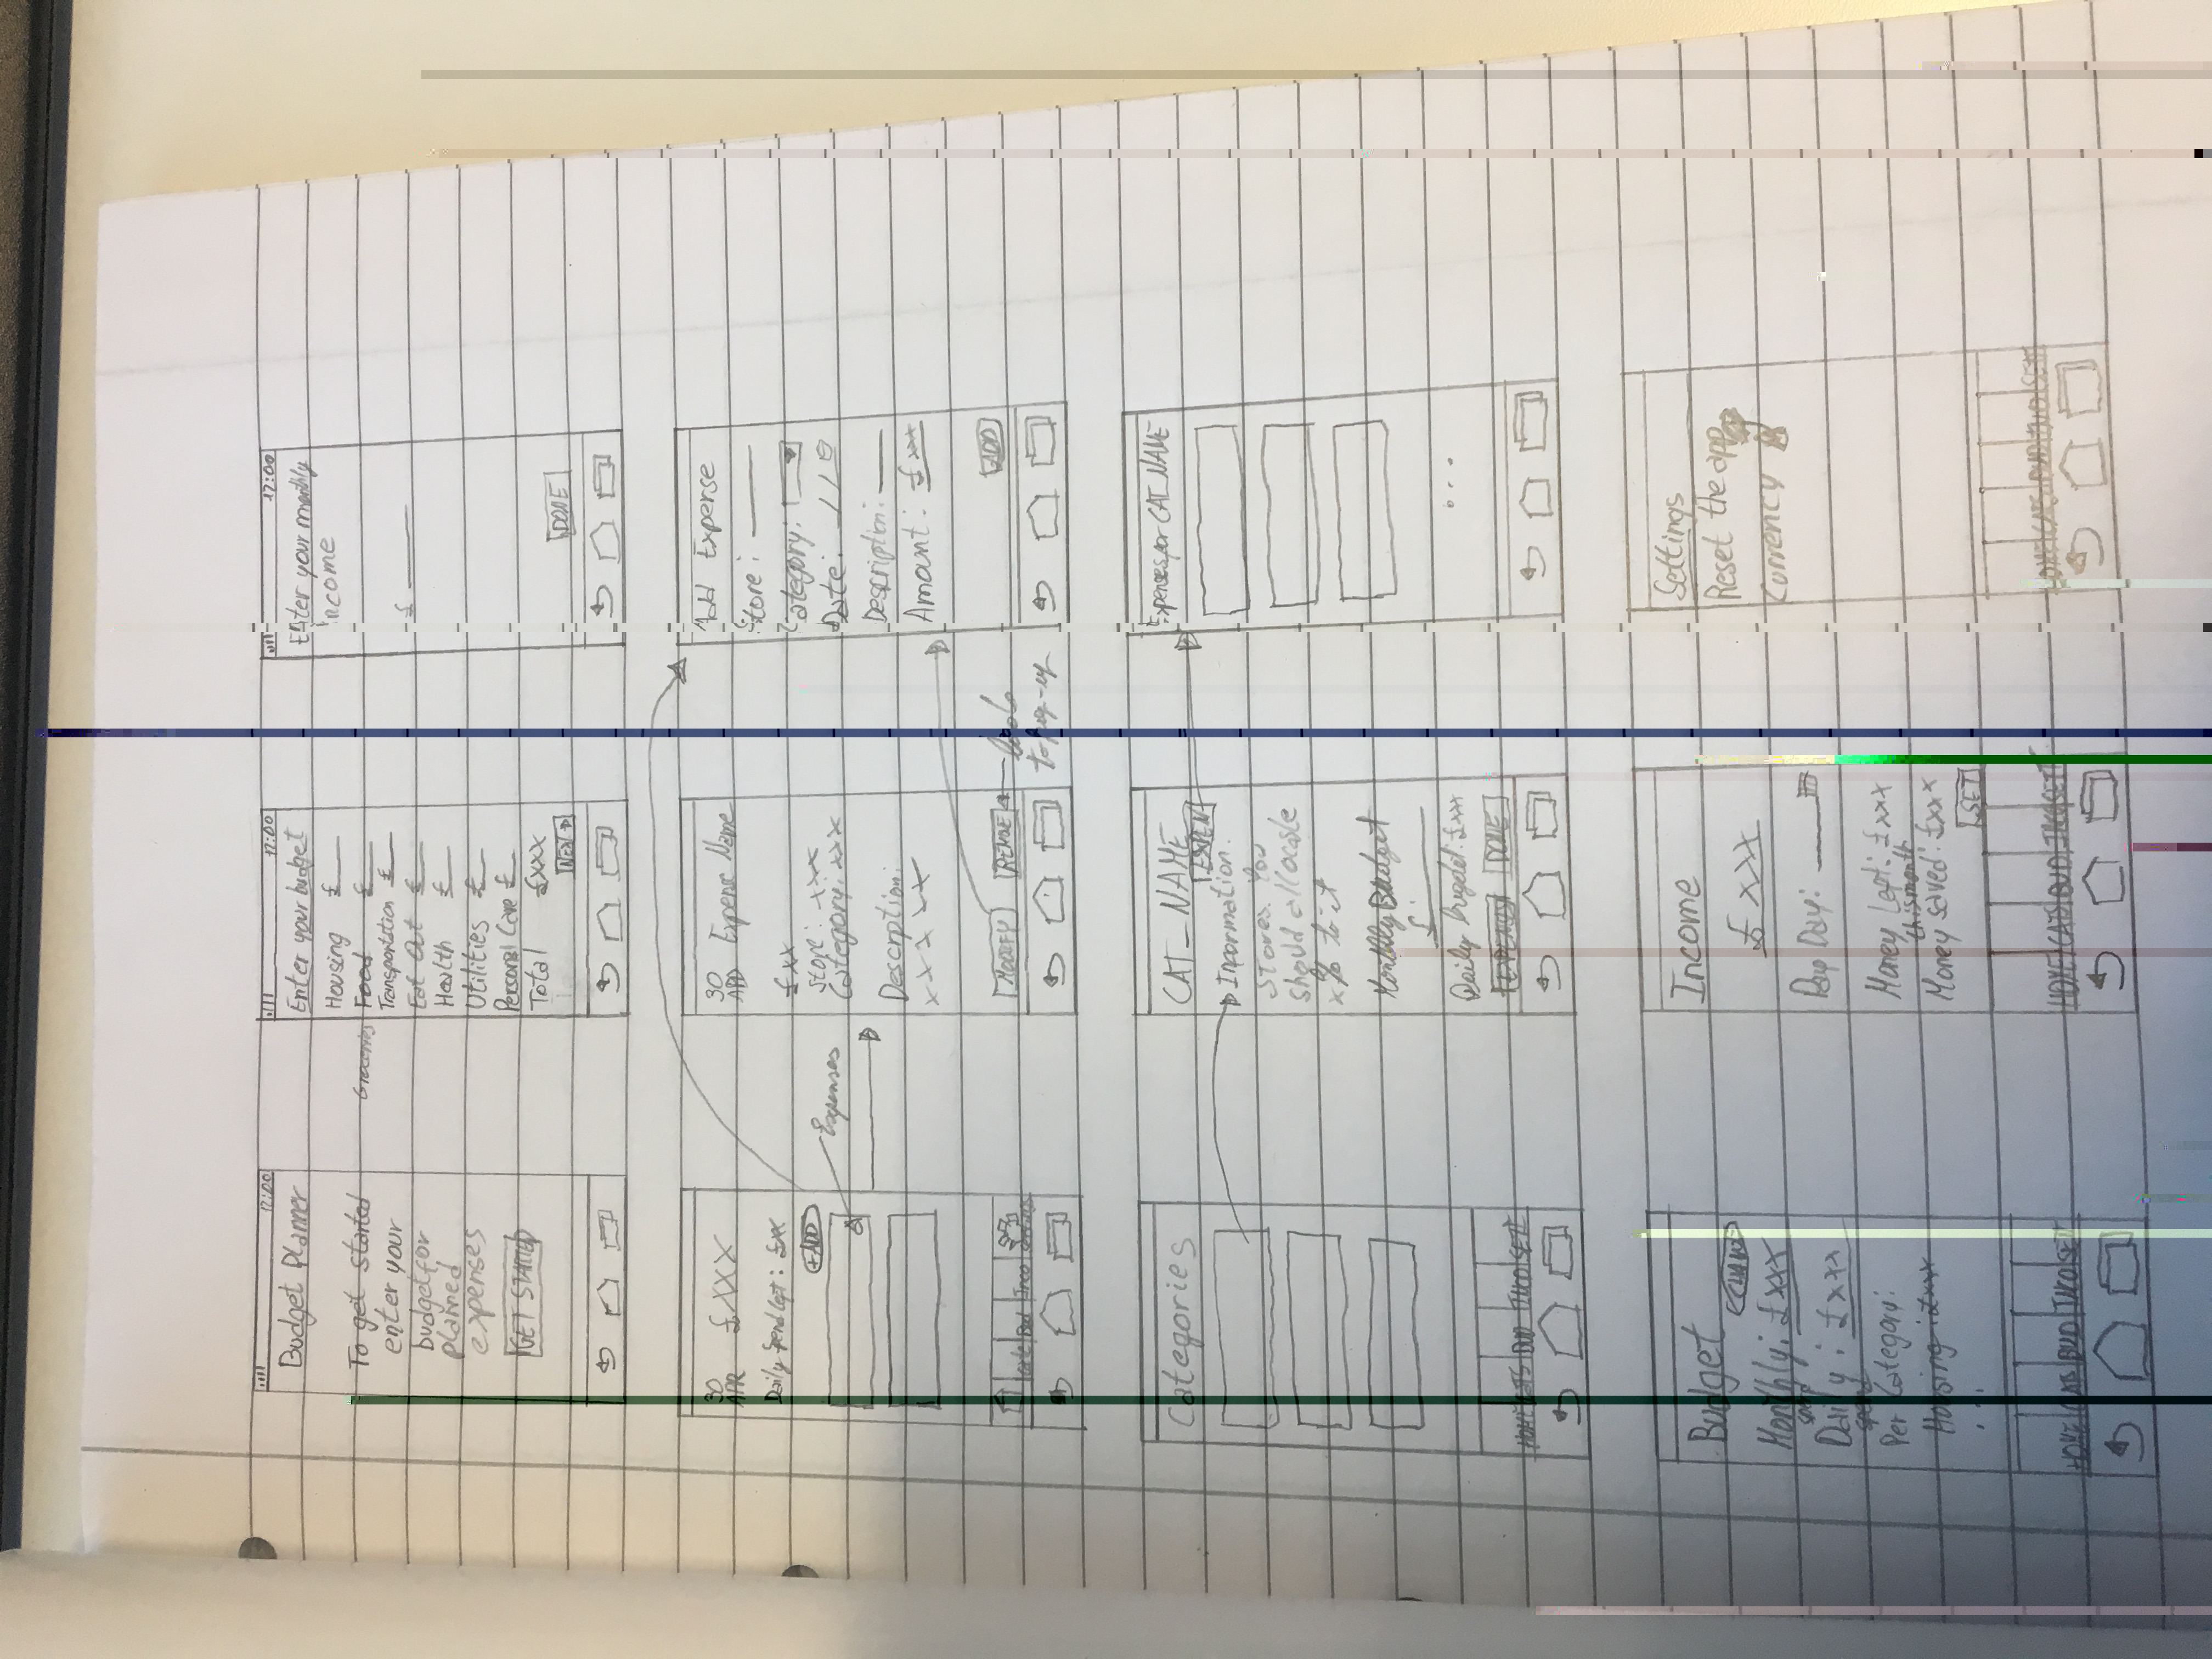
\includegraphics[width=\textwidth]{sketches.jpg}
\end{figure}

\section{Wireframes}
When converting the sketches to wireframes, I used an open-source GUI prototyping tool called \emph{Pencil - add reference here} and elements from collections that contained common Android user interface elements to give them a more realistic look and feel.

\begin{figure}
  \caption{Introduction Screen wireframes}
  \centering
  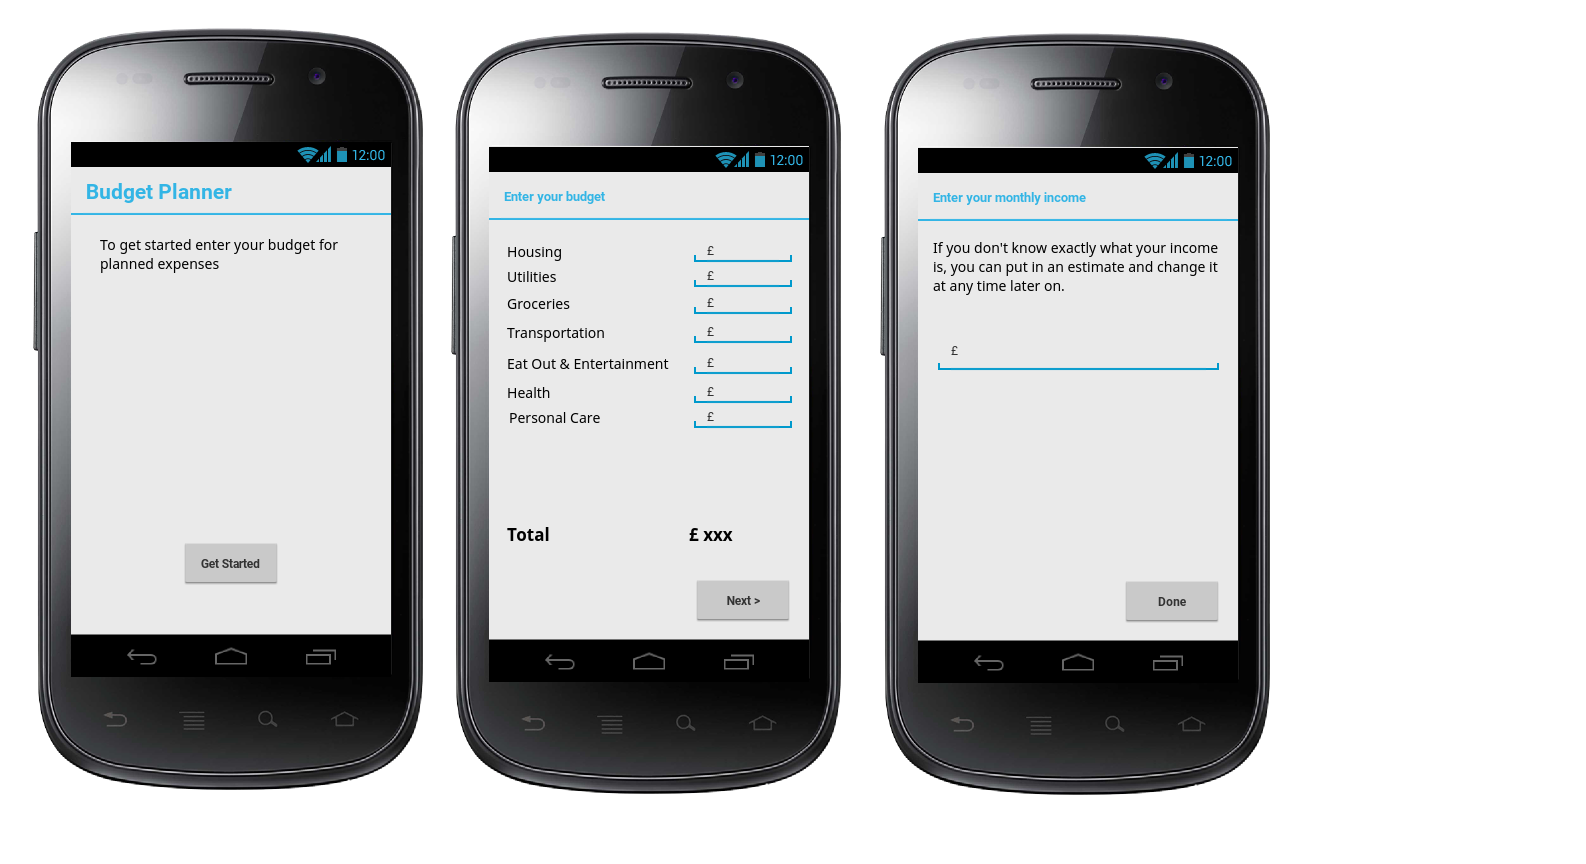
\includegraphics[width=\textwidth]{first_launch.png}
\end{figure}

\begin{figure}
  \caption{Home Screen and expenses-related wireframes}
  \centering
  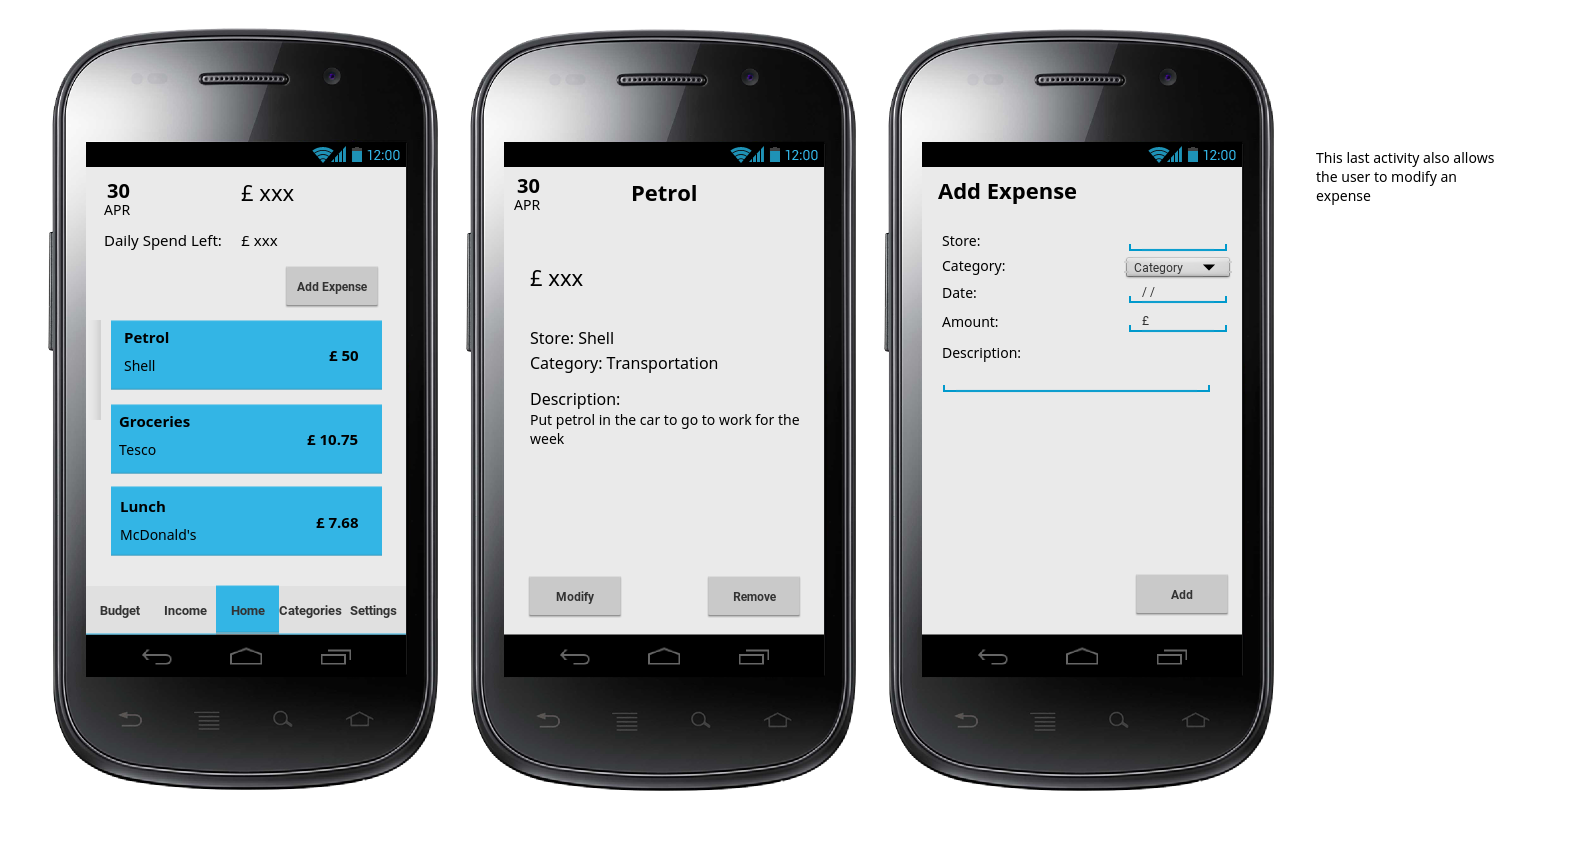
\includegraphics[width=\textwidth]{expenses.png}
\end{figure}

\begin{figure}
  \caption{Category-related views wireframes}
  \centering
  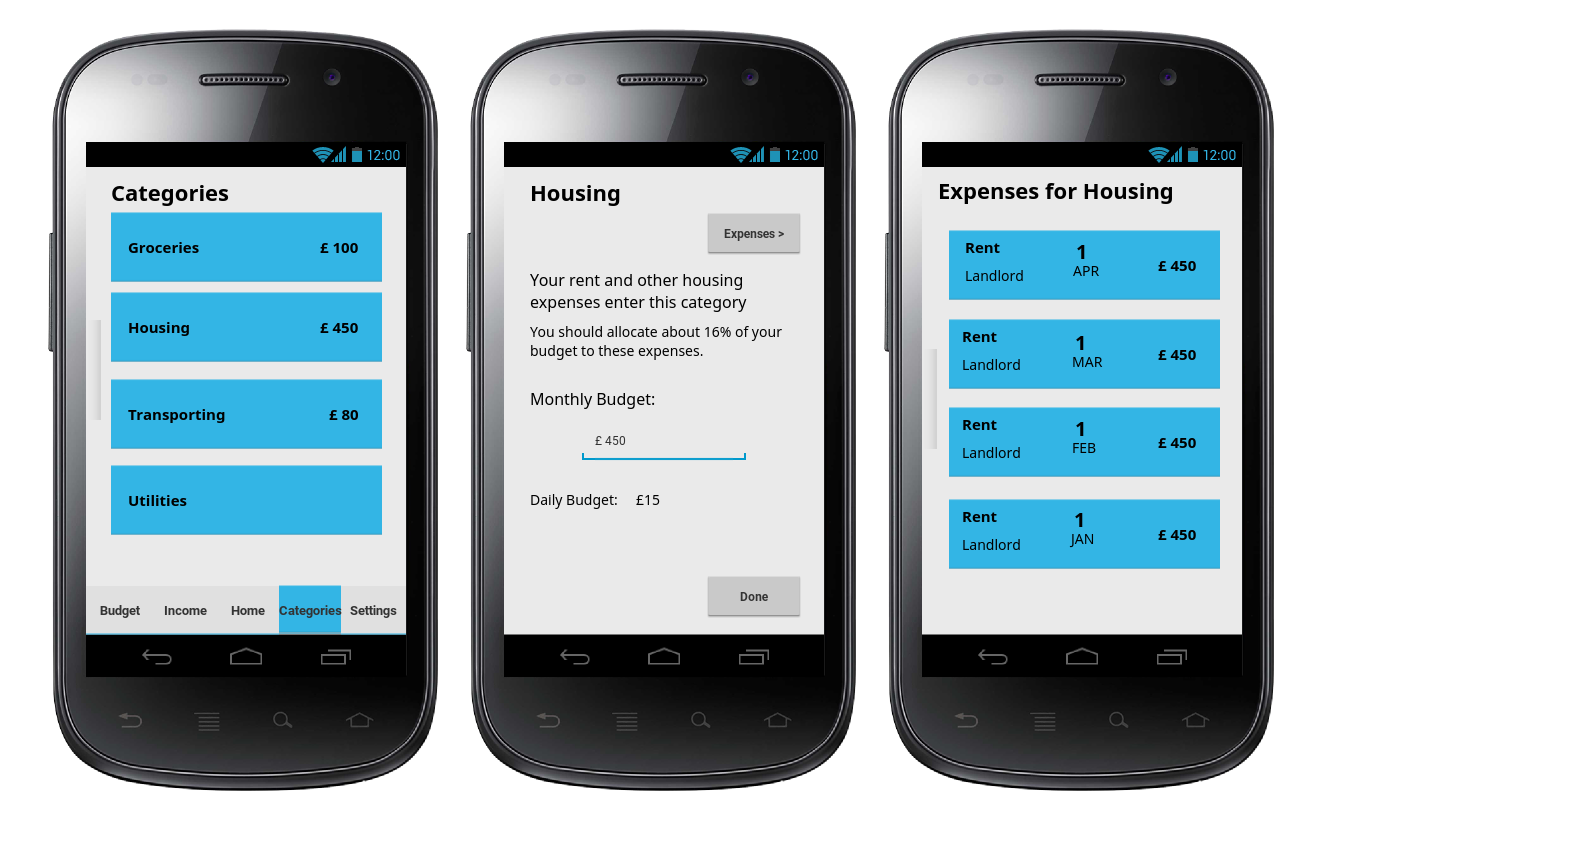
\includegraphics[width=\textwidth]{categories.png}
\end{figure}

\begin{figure}
  \caption{Budget, Income and Settings views wireframes}
  \centering
  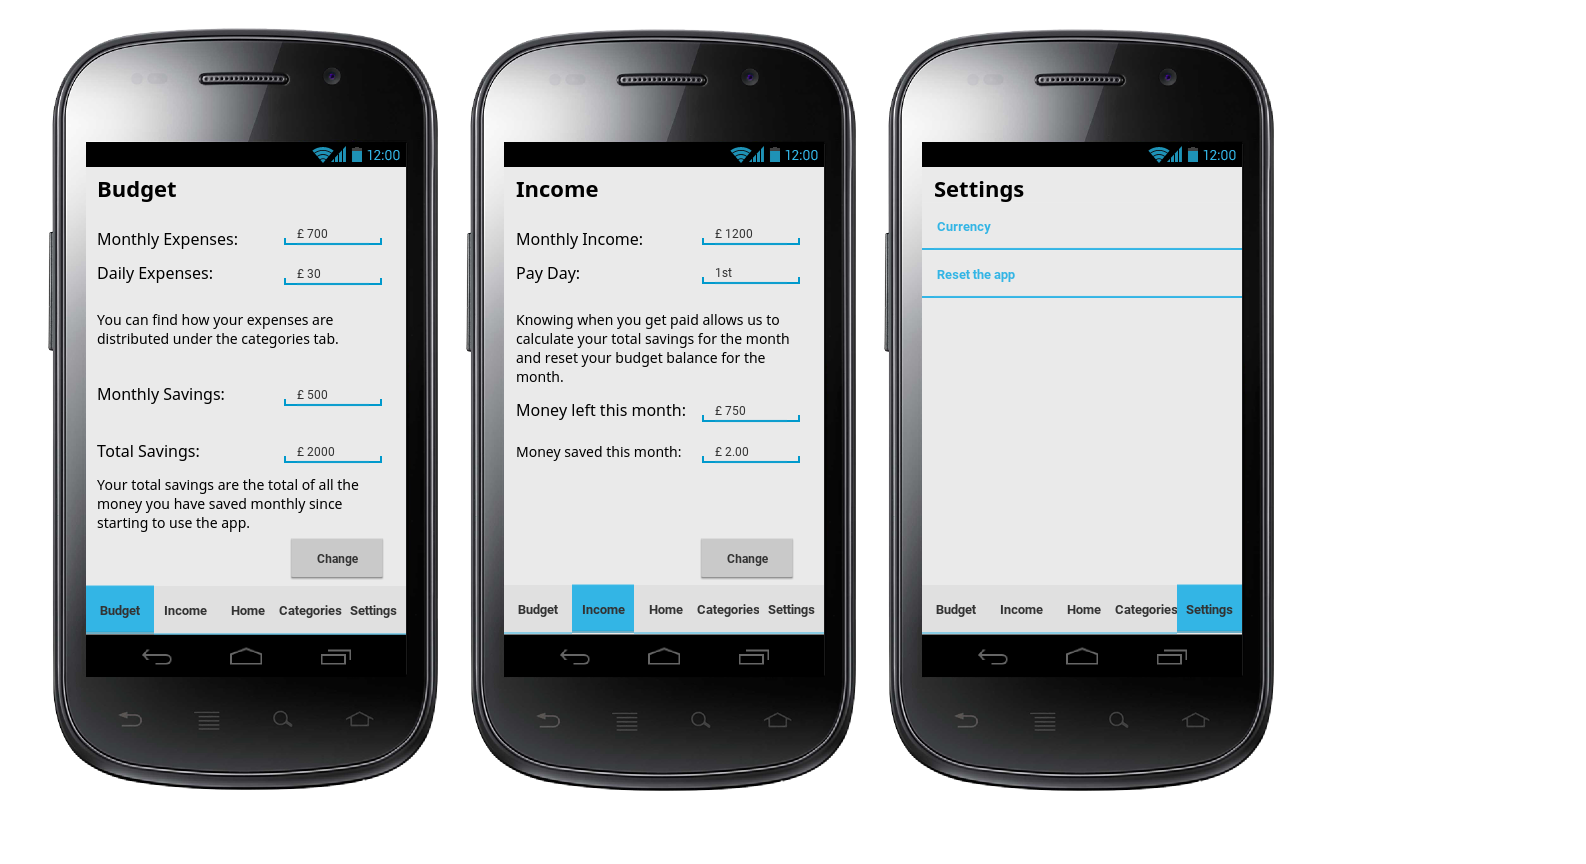
\includegraphics[width=\textwidth]{last_activities.png}
\end{figure}

\section{App Inventor Implementation}
The implementation of the user interface was pretty straightforward, however, there were some things that I needed to take into consideration and work around with when building the interface:
\begin{itemize}
  \item In App Inventor the elements have fixed positions that are automatically allocated in by the system and are not customizable, therefore I had to place different horizontal and vertical arrangements and play with the height and width of the elements to get them positioned where I wanted them to be.
  \item App Inventor doesn't allow certain elements to be clickable or to have certain types of event handlers (which I only realised when trying to implement the programming into the User Interface), therefore I had to spend extra time into customizing the appereance of certain elements such as buttons or lists to get an appearance similar to the one I had originally designed. This wasn't possible for every case, unfortunately, and some elements of the interface do look quite different when compared to the wireframes.
\end{itemize}

Here is the final user interface of the application, as seen in the design screen of App Inventor:

\begin{figure}
  \caption{Introduction Screen}
  \centering
  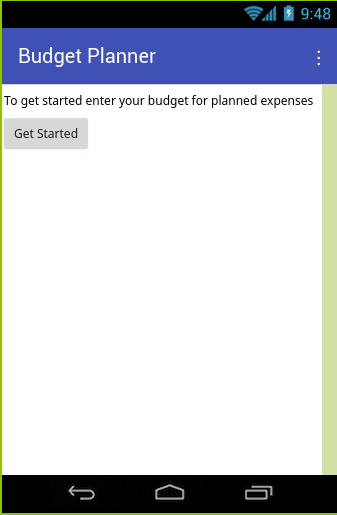
\includegraphics[width=\textwidth]{intro.png}
\end{figure}

\begin{figure}
  \caption{Introduction Budget Input}
  \centering
  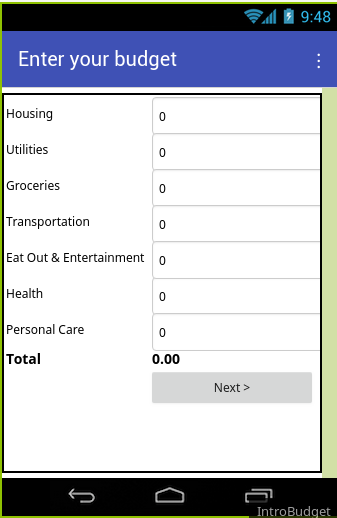
\includegraphics[width=\textwidth]{introBudget.png}
\end{figure}

\begin{figure}
  \caption{Introduction Income Input}
  \centering
  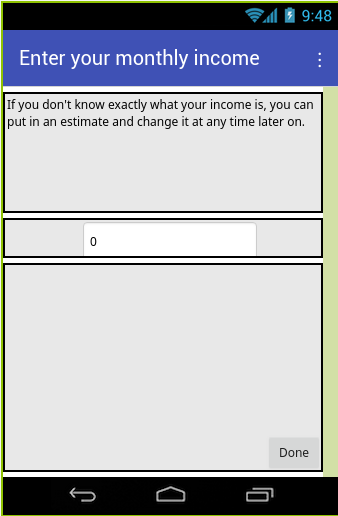
\includegraphics[width=\textwidth]{introIncome.png}
\end{figure}

\begin{figure}
  \caption{Home Screen}
  \centering
  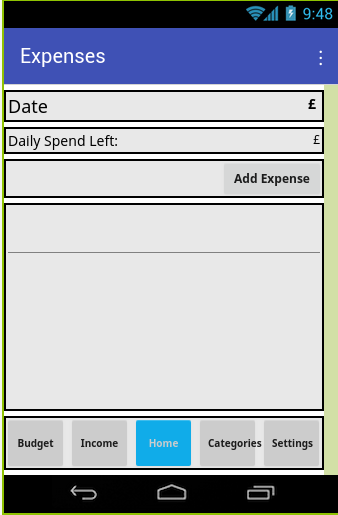
\includegraphics[width=\textwidth]{homeScreen.png}
\end{figure}

\begin{figure}
  \caption{Expense View}
  \centering
  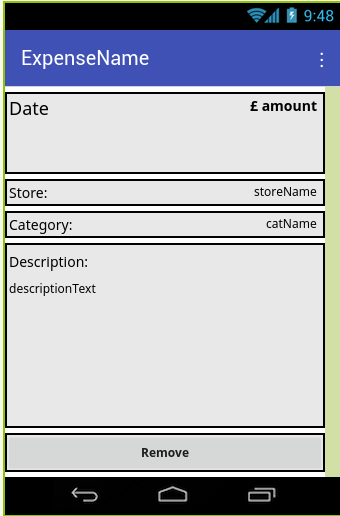
\includegraphics[width=\textwidth]{expenseView.png}
\end{figure}

\begin{figure}
  \caption{Add Expense Screen}
  \centering
  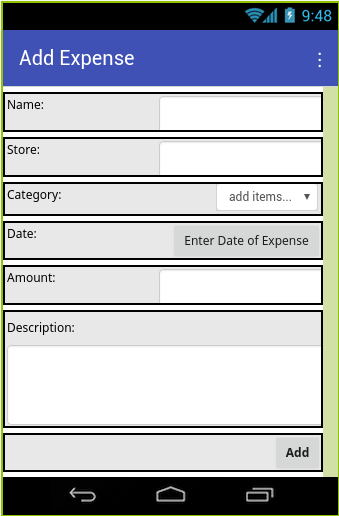
\includegraphics[width=\textwidth]{addExpense.png}
\end{figure}

\begin{figure}
  \caption{Categories List View}
  \centering
  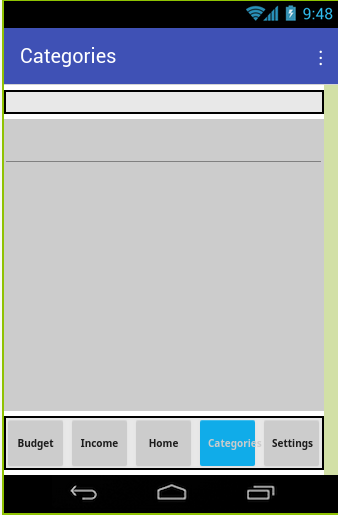
\includegraphics[width=\textwidth]{categoriesView.png}
\end{figure}

\begin{figure}
  \caption{Individual Category View}
  \centering
  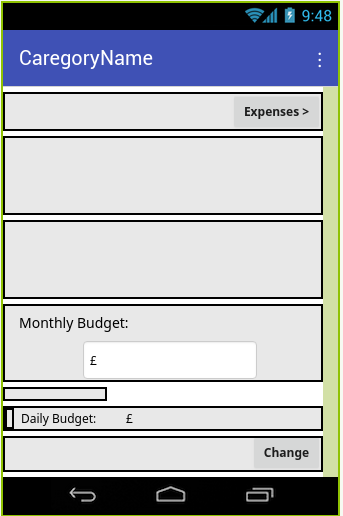
\includegraphics[width=\textwidth]{categoryView.png}
\end{figure}

\begin{figure}
  \caption{Expenses for a Category View}
  \centering
  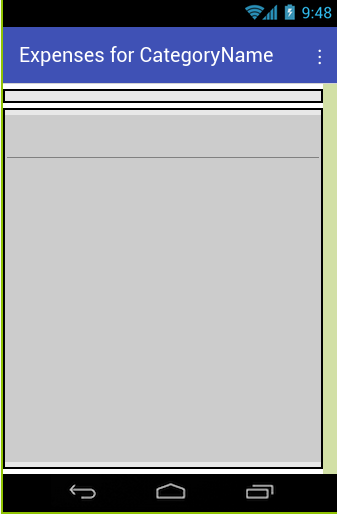
\includegraphics[width=\textwidth]{categoryExpenses.png}
\end{figure}

\begin{figure}
  \caption{Budget View}
  \centering
  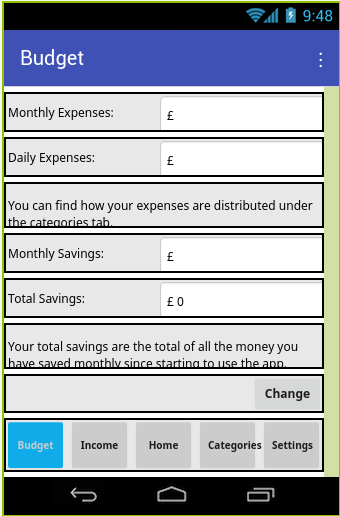
\includegraphics[width=\textwidth]{budget.png}
\end{figure}

\begin{figure}
  \caption{Income View}
  \centering
  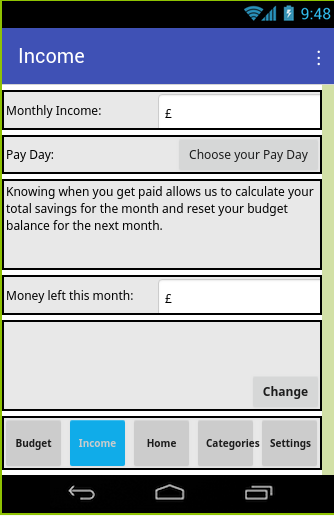
\includegraphics[width=\textwidth]{income.png}
\end{figure}

\begin{figure}
  \caption{Settings View}
  \centering
  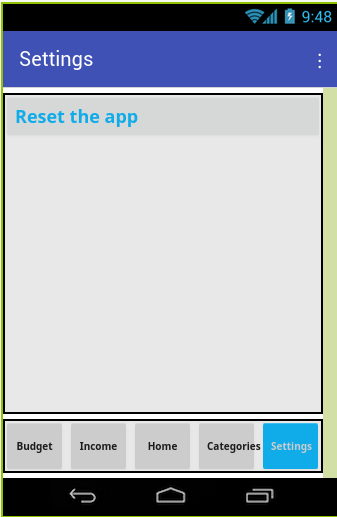
\includegraphics[width=\textwidth]{settings.png}
\end{figure}
